%%%%%%%%%%%%%%%%%%%%%%%%%%%%%%%%%%%%%%%%%
% Short Sectioned Assignment LaTeX Template Version 1.0 (5/5/12)
% This template has been downloaded from: http://www.LaTeXTemplates.com
% Original author:  Frits Wenneker (http://www.howtotex.com)
% License: CC BY-NC-SA 3.0 (http://creativecommons.org/licenses/by-nc-sa/3.0/)
%%%%%%%%%%%%%%%%%%%%%%%%%%%%%%%%%%%%%%%%%

%----------------------------------------------------------------------------------------
%	PACKAGES AND OTHER DOCUMENT CONFIGURATIONS
%----------------------------------------------------------------------------------------

\documentclass[paper=a4, fontsize=11pt]{scrartcl} % A4 paper and 11pt font size

% ---- Entrada y salida de texto -----

\usepackage[T1]{fontenc} % Use 8-bit encoding that has 256 glyphs
\usepackage[utf8]{inputenc}
%\usepackage{fourier} % Use the Adobe Utopia font for the document - comment this line to return to the LaTeX default

% ---- Idioma --------

\usepackage[spanish, es-tabla]{babel} % Selecciona el español para palabras introducidas automáticamente, p.ej. "septiembre" en la fecha y especifica que se use la palabra Tabla en vez de Cuadro

% ---- Otros paquetes ----

\usepackage{url} % ,href} %para incluir URLs e hipervínculos dentro del texto (aunque hay que instalar href)
\usepackage{amsmath,amsfonts,amsthm} % Math packages
%\usepackage{graphics,graphicx, floatrow} %para incluir imágenes y notas en las imágenes
\usepackage{graphics,graphicx, float} %para incluir imágenes y colocarlas

% Para hacer tablas comlejas
%\usepackage{multirow}
%\usepackage{threeparttable}

%\usepackage{sectsty} % Allows customizing section commands
%\allsectionsfont{\centering \normalfont\scshape} % Make all sections centered, the default font and small caps

\usepackage{fancyhdr} % Custom headers and footers
\pagestyle{fancyplain} % Makes all pages in the document conform to the custom headers and footers
\fancyhead{} % No page header - if you want one, create it in the same way as the footers below
\fancyfoot[L]{} % Empty left footer
\fancyfoot[C]{} % Empty center footer
\fancyfoot[R]{\thepage} % Page numbering for right footer
\renewcommand{\headrulewidth}{0pt} % Remove header underlines
\renewcommand{\footrulewidth}{0pt} % Remove footer underlines
\setlength{\headheight}{13.6pt} % Customize the height of the header

\numberwithin{equation}{section} % Number equations within sections (i.e. 1.1, 1.2, 2.1, 2.2 instead of 1, 2, 3, 4)
\numberwithin{figure}{section} % Number figures within sections (i.e. 1.1, 1.2, 2.1, 2.2 instead of 1, 2, 3, 4)
\numberwithin{table}{section} % Number tables within sections (i.e. 1.1, 1.2, 2.1, 2.2 instead of 1, 2, 3, 4)

\setlength\parindent{0pt} % Removes all indentation from paragraphs - comment this line for an assignment with lots of text

\newcommand{\horrule}[1]{\rule{\linewidth}{#1}} % Create horizontal rule command with 1 argument of height

%	TÍTULO Y DATOS DEL ALUMNO
%----------------------------------------------------------------------------------------

\title{	
	\normalfont \normalsize 
	\textsc{\textbf{Planificación y Gestión de Proyectos Informáticos (2018-2019)} \\ Máster Profesional de Ingeniería Informática \\ Universidad de Granada} \\ [25pt] % Your university, school and/or department name(s)
	\horrule{0.5pt} \\[0.4cm] % Thin top horizontal rule
	\huge Ajuste del plan del proyecto \\ % The assignment title
	\horrule{2pt} \\[0.5cm] % Thick bottom horizontal rule
}

\author{Alejandro Campoy Nieves \\ Luis Gallego Quero} % Nombre y apellidos y correo
\date{\normalsize\today} % Incluye la fecha actual

\usepackage[spanish, es-tabla]{babel}
\usepackage{hyperref} % Para añadir los hiperenlaces.
\hypersetup{
	colorlinks=true,
	linkcolor=blue,
	filecolor=magenta,      
	urlcolor=cyan,
}
\usepackage{graphicx}
\usepackage{amssymb, amsmath, amsbsy}
\usepackage{mathptmx}	
\usepackage{float}
\usepackage{booktabs}					%paquete para realización de tablas profesionales
\usepackage{eurosym}
%\usepackage[table]{xcolor}
%\definecolor{lightgray}{gray}{0.9}
\usepackage{xcolor}
\usepackage{colortbl}


%----------------------------------------------------------------------------------------
% DOCUMENTO
%----------------------------------------------------------------------------------------

\begin{document}
	\maketitle % Muestra el Título
	
	\newpage %inserta un salto de página
	
	\tableofcontents % para generar el índice de contenidos
	
	\listoffigures
	
	\listoftables	
	
	\newpage	
 
\section{Riesgos identificados}
\begin{table}[H]
	\begin{center}
		\begin{tabular}{|c||c|c|c|}
			\hline 
			Riesgo & Probabilidad & Impacto(Mejor-Normal-Peor) & Exposición  \\
			\hline \hline
			R1 & 0.1 & 0.15 - 0.3 - 0.6 & 0.03 \\ \hline
			R2 & 0.3 & 0.3 - 0.35 - 0.5 & 0.105 \\ \hline
			R3 & 0.25 & 0.2 - 0.3 - 0.5 & 0.075 \\ \hline
			R4 & 0.15 & 0.1 - 0.15 - 0.2 & 0.0225 \\ \hline
			R5 & 0.15 & 0.3 - 0.45 - 0.6 & 0.0675 \\ \hline
			R6 & 0.15 & 0.1 - 0.25 - 0.3 & 0.0375 \\ \hline
			R7 & 0.2 & 0.1 - 0.2 - 0.4 & 0.04 \\ \hline
			R8 & 0.05 & 0.05 - 0.2 - 0.5 & 0.01 \\ \hline
			R9 & 0.1 & 0.05 - 0.1 - 0.2  & 0.01 \\ \hline
			R10 & 0.3 & 0.2 - 0.35 - 0.7 & 0.105 \\ \hline \hline
			\textbf{Total} & & & 0.5025 \\ \hline
		\end{tabular}
		\caption{Tabla de riesgos}
		\label{tabla:riesgos}
	\end{center}
\end{table}

\section{Estimación del impacto del proyecto}

\begin{figure}[h]
	\centering 		
	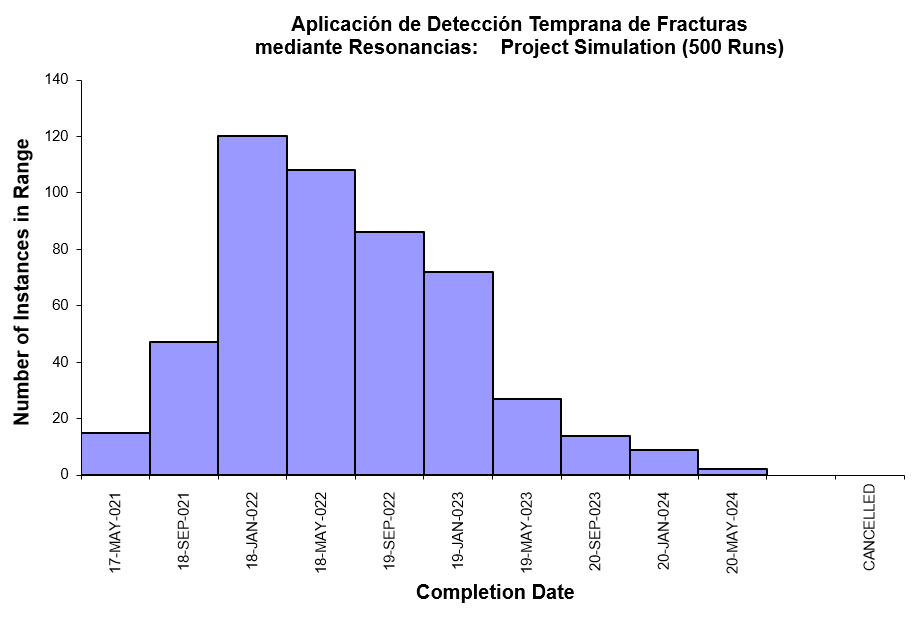
\includegraphics[scale=0.7]{figura1.png}
	\caption{Simulación de impacto del proyecto con herramienta Riskology.}
	\label{fig:riskology} 
\end{figure}

La estimación del proyecto según Riskology asciende a un par de años más de lo que habíamos estimado, lo que nos parece excesivo. Por otra parte, nos sale que la probabilidad de que se cancele el proyecto es nula teniendo en cuenta los riesgos expuestos.

\section{Ajuste de estimaciones y conclusión final}

Como determinamos en la práctica perteneciente a los presupuestos, necesitamos un total de 51.000 euros para llevar a cabo nuestro proyecto. Sin embargo, teniendo en cuenta el 50,25 \% de exposición a los riesgos contemplados, el coste final del proyecto ascendería a los \textbf{76.627,5 euros} para tener cubiertos todos los riesgos posibles a los que nos encontramos expuestos.





%\newpage
%\bibliographystyle{plain}
%\bibliography{biblio}

\end{document}       
%---------------------------------------------------
